\RequirePackage{fix-cm}
\documentclass{article}
\usepackage[papersize={80cm,110cm},vmargin=.08\paperheight,hmargin=.09\paperwidth]{geometry}
\usepackage{nopageno}
\usepackage{mathpazo,courier,helvet}

  \renewcommand{\familydefault}{\sfdefault}
  \renewcommand{\tiny}{\fontsize{12}{14}\selectfont}
  \renewcommand{\scriptsize}{\fontsize{14.4}{18}\selectfont}
  \renewcommand{\footnotesize}{\fontsize{17.28}{22}\selectfont}
  \renewcommand{\small}{\fontsize{20.74}{25}\selectfont}
  \renewcommand{\normalsize}{\fontsize{24.88}{30}\selectfont}
  \renewcommand{\large}{\fontsize{29.86}{37}\selectfont}
  \renewcommand{\Large}{\fontsize{35.83}{45}\selectfont}
  \renewcommand{\LARGE}{\fontsize{43}{54}\selectfont}
  \renewcommand{\huge}{\fontsize{51.6}{64}\selectfont}
  \renewcommand{\Huge}{\fontsize{61.92}{77}\selectfont}
  \newcommand{\veryHuge}{\fontsize{74.3}{93}\selectfont}
  \newcommand{\VeryHuge}{\fontsize{85}{112}\selectfont}
  \newcommand{\VERYHuge}{\fontsize{90}{130}\selectfont}
  \renewcommand{\normalsize}{\fontsize{26}{34}\selectfont}
\def\nodetextsize{\Large}

%\usepackage[T1]{fontenc}
%\usepackage{microtype}
\usepackage{url}
\usepackage{adjustbox}
\usepackage{amsmath,amssymb,amsfonts} 
\usepackage{amsthm}
\usepackage{mathtools}
%\usepackage{mathptmx}
\usepackage{nicefrac}
\usepackage{fancybox}
\usepackage{tikz}
\usepackage{pgfplots}
\pgfplotsset{compat=newest,xtick={0,10,...,110}}

\usepackage{bm}
\usepackage{graphicx}
\usepackage{ifthen}
\usepackage{multicol}
\usepackage{color}
%\usepackage[usenames,dvipsnames]{xcolor}{ProcessBlue}
%\setlength{\columnseprule}{1pt}

\setlength{\columnsep}{2cm}

\DeclareGraphicsExtensions{.pdf,.png,.jpg}

\usepackage{tikz}
\usetikzlibrary{calc,matrix,plotmarks,trees,arrows,automata}
\usetikzlibrary{shapes.geometric}
\usetikzlibrary{fit}
\usetikzlibrary{backgrounds}
\tikzset{
    triangle/.style={
        draw,
        regular polygon,
        regular polygon sides=3,
        node distance=3cm,
        minimum height=5cm
    }
}

\DeclareMathOperator{\len}{len}
\DeclareMathOperator{\trans}{T}
\DeclareMathOperator{\atrans}{S}
\DeclarePairedDelimiter{\group}{(}{)}
\DeclarePairedDelimiter{\sqgroup}{[}{]}
\DeclarePairedDelimiter{\set}{\{}{\}}
\DeclarePairedDelimiter{\avg}{\langle}{\rangle}
\DeclarePairedDelimiter{\norm}{\Vert}{\Vert}
\DeclarePairedDelimiter{\abs}{\vert}{\vert}
\DeclarePairedDelimiter{\floor}{\lfloor}{\rfloor}


\newcommand{\Y}{\mathcal{Y}}

\newcommand{\asa}{\Leftrightarrow}

\newcommand{\gambles}{\mathcal{L}}
\newcommand{\gamblesX}{\gambles(\states)} 

\newcommand{\rateset}{\mathcal{Q}}
\newcommand{\lrate}{\underline{Q}}

\newcommand{\nat}{\mathbb{N}}
\newcommand{\our}{\emph{Geo/Geo/1/L} }
\newcommand{\arr}{$[\underline{a},\overline{a}]$ }
\newcommand{\dep}{$[\underline{d},\overline{d}]$ }

\newcommand{\lp}[1]{\underline{#1}}
\newcommand{\up}[1]{\overline{#1}}
\newcommand{\matrices}{\mathcal{Q}}
\newcommand{\lmatrixi}[1]{\underline{\matrices}_{#1}}
\newcommand{\umatrixi}[1]{\overline{\matrices}_{#1}}

\newcommand{\lx}[1]{\breve{#1}}
\newcommand{\ux}[1]{\hat{#1}}
\newcommand{\lxd}[1]{{#1}^{\ast}}
\newcommand{\uxd}[1]{{#1}^{\diamond}}

\newcommand{\timeft}[2]{\tau_{#1\to#2}}
\newcommand{\timeftarg}[3]{\tau_{#1\to#2}(#3)}
\newcommand{\ltimeft}[2]{\underline{\tau}_{#1\to#2}}
\newcommand{\utimeft}[2]{\overline{\tau}_{#1\to#2}}
\newcommand{\prm}[1]{#1^{\prime}}

\newcommand{\statesymbol}{X}
\newcommand{\statessymbol}{\mathcal{X}}
\newcommand{\gamblessymbol}{\mathcal{G}}

\newcommand{\state}[1]{\statesymbol_{#1}}
\newcommand{\xval}[1]{x_{#1}}
\newcommand{\states}[1]{\statessymbol_{#1}}
\newcommand{\stateset}{\statessymbol}
%\newcommand{\normedgambles}[1]{\gamblessymbol_1(\states{#1})}
\newcommand{\stateto}[1]{\state{1:#1}}
\newcommand{\statefrom}[1]{\state{#1:}}
\newcommand{\statefromto}[2]{\state{#1:#2}}
\newcommand{\xvalto}[1]{\xval{1:#1}}
\newcommand{\xvalfrom}[1]{\xval{#1:}}
\newcommand{\xvalfromto}[2]{\xval{#1:#2}}
\newcommand{\statesto}[1]{\states{1:#1}}
\newcommand{\statesfrom}[1]{\states{#1:}}
\newcommand{\statesfromto}[2]{\states{#1:#2}}
\newcommand{\gamblesto}[1]{\gamblessymbol(\states{1:#1})}
\newcommand{\gamblesfrom}[1]{\gamblessymbol(\states{#1:})}
\newcommand{\gamblesfromto}[2]{\gamblessymbol(\states{#1:#2})}

\newcommand{\nats}{\mathbb{N}}
\newcommand{\natswithzero}{\mathbb{N}_0}
\newcommand{\reals}{\mathbb{R}}

\newcommand{\init}{\square}
\newcommand{\pth}{\omega}
\newcommand{\sits}{\pths^\lozenge}
\newcommand{\pths}{\Omega}

\newcommand{\ex}{E}
\newcommand{\lex}{\underline{\ex}}
\newcommand{\uex}{\overline{\ex}}
\newcommand{\aex}{F}
\newcommand{\alex}{\underline{\aex}}
\newcommand{\auex}{\overline{\aex}}
\newcommand{\aaex}{Q}
\newcommand{\aalex}{\underline{\aaex}}
\newcommand{\aauex}{\overline{\aaex}}

\newcommand{\pr}{P}
\newcommand{\lpr}{\underline{\pr}}
\newcommand{\upr}{\overline{\pr}}

\newcommand{\joint}[1][]{\ex_{#1}}
\newcommand{\ljoint}[1][]{\lex_{#1}}
\newcommand{\ujoint}[1][]{\uex_{#1}}

\newcommand{\local}[3][]{\aaex\group[#1]{#2#1\vert\stateto{#3}}}
\newcommand{\llocal}[3][]{\aalex\group[#1]{#2#1\vert\stateto{#3}}}
\newcommand{\ulocal}[3][]{\aauex\group[#1]{#2#1\vert\stateto{#3}}}
\newcommand{\xinlocal}[3][]{\aaex\group[#1]{#2#1\vert\xvalto{#3}}}
\newcommand{\xinllocal}[3][]{\aalex\group[#1]{#2#1\vert\xvalto{#3}}}
\newcommand{\xinulocal}[3][]{\aauex\group[#1]{#2#1\vert\xvalto{#3}}}
\newcommand{\sitinlocal}[3][]{\aaex\group[#1]{#2#1\vert#3}}
\newcommand{\sitinllocal}[3][]{\aalex\group[#1]{#2#1\vert#3}}
\newcommand{\sitinulocal}[3][]{\aauex\group[#1]{#2#1\vert#3}}
\newcommand{\margin}[2][]{\aaex\group[#1]{#2#1\vert\init}}
\newcommand{\lmargin}[2][]{\aalex\group[#1]{#2#1\vert\init}}
\newcommand{\umargin}[2][]{\aauex\group[#1]{#2#1\vert\init}}
\newcommand{\transition}[3][]{\aaex\group[#1]{#2#1\vert#3}}
\newcommand{\ltransition}[3][]{\aalex\group[#1]{#2#1\vert#3}}
\newcommand{\utransition}[3][]{\aauex\group[#1]{#2#1\vert#3}}
\newcommand{\glob}[3][]{\ex\group[#1]{#2#1\vert\stateto{#3}}}
\newcommand{\lglobal}[3][]{\lex\group[#1]{#2#1\vert\stateto{#3}}}
\newcommand{\uglobal}[3][]{\uex\group[#1]{#2#1\vert\stateto{#3}}}
\newcommand{\xinglobal}[3][]{\ex\group[#1]{#2#1\vert\xvalto{#3}}}
\newcommand{\xinlglobal}[3][]{\lex\group[#1]{#2#1\vert\xvalto{#3}}}
\newcommand{\xinuglobal}[3][]{\uex\group[#1]{#2#1\vert\xvalto{#3}}}
\newcommand{\sitinglobal}[3][]{\ex\group[#1]{#2#1\vert#3}}
\newcommand{\sitinlglobal}[3][]{\lex\group[#1]{#2#1\vert#3}}
\newcommand{\sitinuglobal}[3][]{\uex\group[#1]{#2#1\vert#3}}
\newcommand{\newlglobal}[3]{\lex_{\vert#1}(#2\vert#3)}
\newcommand{\newuglobal}[3]{\uex_{\vert#1}(#2\vert#3)}

\newcommand{\exact}[1]{\Gamma(#1)}

\newcommand{\ltrans}{\underline{\trans}\,}
\newcommand{\utrans}{\overline{\trans}\,}
\newcommand{\latrans}{\underline{\atrans}}

\newcommand{\process}{\mathcal{F}}
\newcommand{\submartin}{\mathcal{M}}
\newcommand{\supermartin}{\mathcal{M}}
\newcommand{\esupermartin}{\supermartin^*}
\newcommand{\test}{\mathcal{T}}
\newcommand{\gambleprocess}{\mathcal{D}}
\newcommand{\summed}[1]{\mathcal{I}^{#1}}

\newcommand{\gain}[1]{\mathcal{W}[#1]}
\newcommand{\avgain}[1]{\avg{\mathcal{W}}[#1]}
\newcommand{\ergodic}[1]{\mathcal{A}[#1]}

\newcommand{\martins}{\mathbb{M}}
\newcommand{\submartins}{\underline{\martins}}
\newcommand{\supermartins}{\overline{\martins}}
\newcommand{\esupermartins}{\supermartins^*}

\newcommand{\coe}{\rho}
\newcommand{\varnorm}[2][]{\norm[#1]{#2}_{\mathrm{v}}}
\newcommand{\cset}[2]{\set{#1\colon#2}}
\newcommand{\ind}[1]{\mathbb{I}_{#1}}
\newcommand{\then}{\Rightarrow}
\newcommand{\neht}{\Leftarrow}
\newcommand{\ifandonlyif}{\Leftrightarrow}
\newcommand{\solp}{\mathfrak{M}}
\newcommand{\andstate}{\,\cdot}
\newcommand{\andpath}{\,\bullet}

\newcommand{\de}{\delta}
\newcommand{\ve}{\varepsilon}

\newcommand{\pflike}{Perron--Frobenius-like}

\newtheorem{theorem}{Theorem}
\newtheorem{proposition}[theorem]{Proposition}
\newtheorem{lemma}[theorem]{Lemma}
\newtheorem{corollary}[theorem]{Corollary}
\newtheorem{definition}{Definition}
\theoremstyle{definition}
\newtheorem{example}{Example}

\newtheorem{Theorem}{Theorem}
\newtheorem{Definition}{Definition}

\newtheorem{assumption}{Assumption}

\newcommand{\afstandknopen}{9 cm}
\newcommand{\afstandkleinepijl}{.8 cm}
\newcommand{\korterkleinepijl}{3.2 cm}
\newcommand{\afstandvollelijn}{3.8 cm}
\newcommand{\afstandomcirkel}{5.6 cm}

\newcommand{\schaal}{3.68}
\newcommand{\schaalb}{3.68}
\newcommand{\schaalC}{1.5}

%TIKZ
\xdefinecolor{red}{RGB}{241, 90, 34}
\xdefinecolor{geel}{RGB}{255, 197, 11}
\xdefinecolor{rose}{RGB}{236, 0, 140}
\xdefinecolor{green}{RGB}{179, 211, 53}
\xdefinecolor{grey}{RGB}{72, 119, 116}
%\xdefinecolor{grijsA}{RGB}{184,169,134}
\xdefinecolor{greyA}{RGB}{115,114,117}
\xdefinecolor{greyB}{RGB}{240,227,197}
%\xdefinecolor{grijstekst}{RGB}{122,99,44}
%\xdefinecolor{grijstekst}{RGB}{115,114,117}
\xdefinecolor{greytext}{RGB}{110, 215, 130}
\xdefinecolor{blackA}{RGB}{199,169,169}
\xdefinecolor{geelA}{RGB}{176,146,26}
\xdefinecolor{blackB}{RGB}{159,212,219}
\xdefinecolor{blackC}{RGB}{120,194,204}
\xdefinecolor{blackD}{RGB}{218,237,240}
\xdefinecolor{blackE}{RGB}{38,126,199}
\xdefinecolor{blacktext}{RGB}{39,146,161}
\xdefinecolor{greenA}{RGB}{41,77,56}
\xdefinecolor{greenB}{RGB}{47,115,21}
\xdefinecolor{redA}{RGB}{209,10,60}
\xdefinecolor{redB}{RGB}{181,25,25}
\definecolor{boeioranje}{RGB}{255,0,0}
%\definecolor{boeiblauw}{RGB}{0,0,255}
\xdefinecolor{boeiblauw}{RGB}{39,146,161}

\colorlet{bijschriftkleur}{black!70}

\tikzstyle{pijl1}=[draw=geel!0!black,line width=.6pt, postaction={decorate}, decoration={markings,mark=at position 1.0 with {\arrow[draw=groen!0!black,line width=10pt]{stealth}}}] 
\tikzstyle{pijl2}=[draw=groen!50!black,line width=.6pt, postaction={decorate}, decoration={markings,mark=at position 1.0 with {\arrow[draw=groen!50!black,line width=1pt]{>}}}]
\tikzstyle{pijl3}=[dashed,line width=0.6pt]
\tikzstyle{pijl4}=[draw=geel!0!black,line width=0.6pt]
\tikzstyle{pijl5}=[draw=bijschriftkleur,dashed,line width=.6pt]
\tikzstyle{pijl1kleur}=[draw=bijschriftkleur,line width=.6pt, postaction={decorate}, decoration={markings,mark=at position 1.0 with {\arrow[bijschriftkleur,line width=0.5pt]{triangle 60}}}] 
%\tikzstyle{knoopobservatie}=[circle,draw=grijsA!50!black,fill=grijsA!99!black,minimum size=3.6cm,line width=.6pt]
\tikzstyle{knoopobservatie}=[circle,draw=groen!50!black,fill=groen,minimum size=3.6cm,line width=.6pt]
\tikzstyle{doelknoop}=[circle,draw=blauwC!30!black,fill=blauwC!70!black,minimum size=3.6cm,line width=.6pt]
\tikzstyle{knoopnietobservatie}=[circle,draw=blauwB!30!black,fill=blauwB!70!black,minimum size=3.6cm,line width=.6pt]
\tikzstyle{knoopbijschrift}=[rectangle, text width=8em, draw=bijschriftkleur, densely dotted, minimum height=.4cm, minimum size=.45cm,  line width=.6pt, fill=blue!0!white, text centered, rounded corners]
\tikzstyle{knoopzonderrand}=[draw=none,fill=none]
\tikzstyle{knoopwit}=[circle,draw=black!100,fill=geel!0,minimum size=3.0cm,line width=.6pt]
\tikzstyle{omcirkelemissiemodel}=[grijsA!70!black,fill=grijstekst!50!white,rounded corners=0.2cm, line width=.6pt] 
\tikzstyle{omcirkeltransitiemodel}=[blauwC,fill=blauwD,rounded corners=0.2cm, line width=.6pt] 
\tikzstyle{omcirkelHMM}=[groenA,fill=none,rounded corners=1cm, dash pattern= on 25pt off 15pt, line width=5pt] 
%\tikzstyle{bolletje}=[circle,roodA,fill=roodA,fill opacity=0.8,minimum size=0.5cm] 
\tikzstyle{bolletje}=[circle,boeioranje,fill=boeioranje,fill opacity=0.6,minimum size=0.5cm] 


\definecolor{UGentblauw}{cmyk}{1,.8,.3,.05}
\definecolor{UGentgeel}{cmyk}{0,.3,1,0}
\tikzstyle{simplexbackground}=[UGentblauw,fill=UGentblauw!5,text=black,rounded corners=.0cm]
%\tikzstyle{bluebackground}=[very thin,draw=blauwE!30!black,fill=blauwE!70!black,fill opacity=0.6,rounded corners=.0cm]
\tikzstyle{bluebackground}=[very thin,draw=boeiblauw!70!black,fill=boeiblauw,fill opacity=0.6,rounded corners=.0cm]
\tikzstyle{blackbackground}=[very thin,draw=darkgray,fill=gray,fill opacity=.6,rounded corners=.000cm]
%\tikzstyle{blackbackground}=[very thin,draw=darkgray,fill=grijsA!70!black,fill opacity=1,rounded corners=.000cm]
%\tikzstyle{yellowbackground}=[very thin,draw=darkgray,fill=grijsA!70!black,fill opacity=1,rounded corners=.000cm]
\tikzstyle{yellowbackground}=[very thin,draw=darkgray,fill=gray,fill opacity=.6,rounded corners=.000cm]
%\tikzstyle{redbackground}=[very thin,draw=roodA!70!black,fill=roodA,fill opacity=0.6,rounded corners=.0000cm]
\tikzstyle{redbackground}=[very thin,draw=boeioranje!70!black,fill=boeioranje,fill opacity=0.6,rounded corners=.0000cm]
\tikzstyle{simplexborder}=[UGentblauw!60,rounded corners=.0cm]


\begin{document}

\thispagestyle{empty}
\def\afstand{7} % afstand tussen de nodes van de boom
\def\hmmafstand{6} % afstand tussen de nodes van de HMM
\def\mesoffset{14pt} % afstand tussen een edge en het pijltje van de message
\def\nodetextsize{\Large} % tekstgrootte van de nodes
\def\titletextsize{\LARGE} % tekstgrootte van de titels
\newcommand{\titlemessagetextsize}{\fontsize{28}{30}\selectfont}

\begin{center}
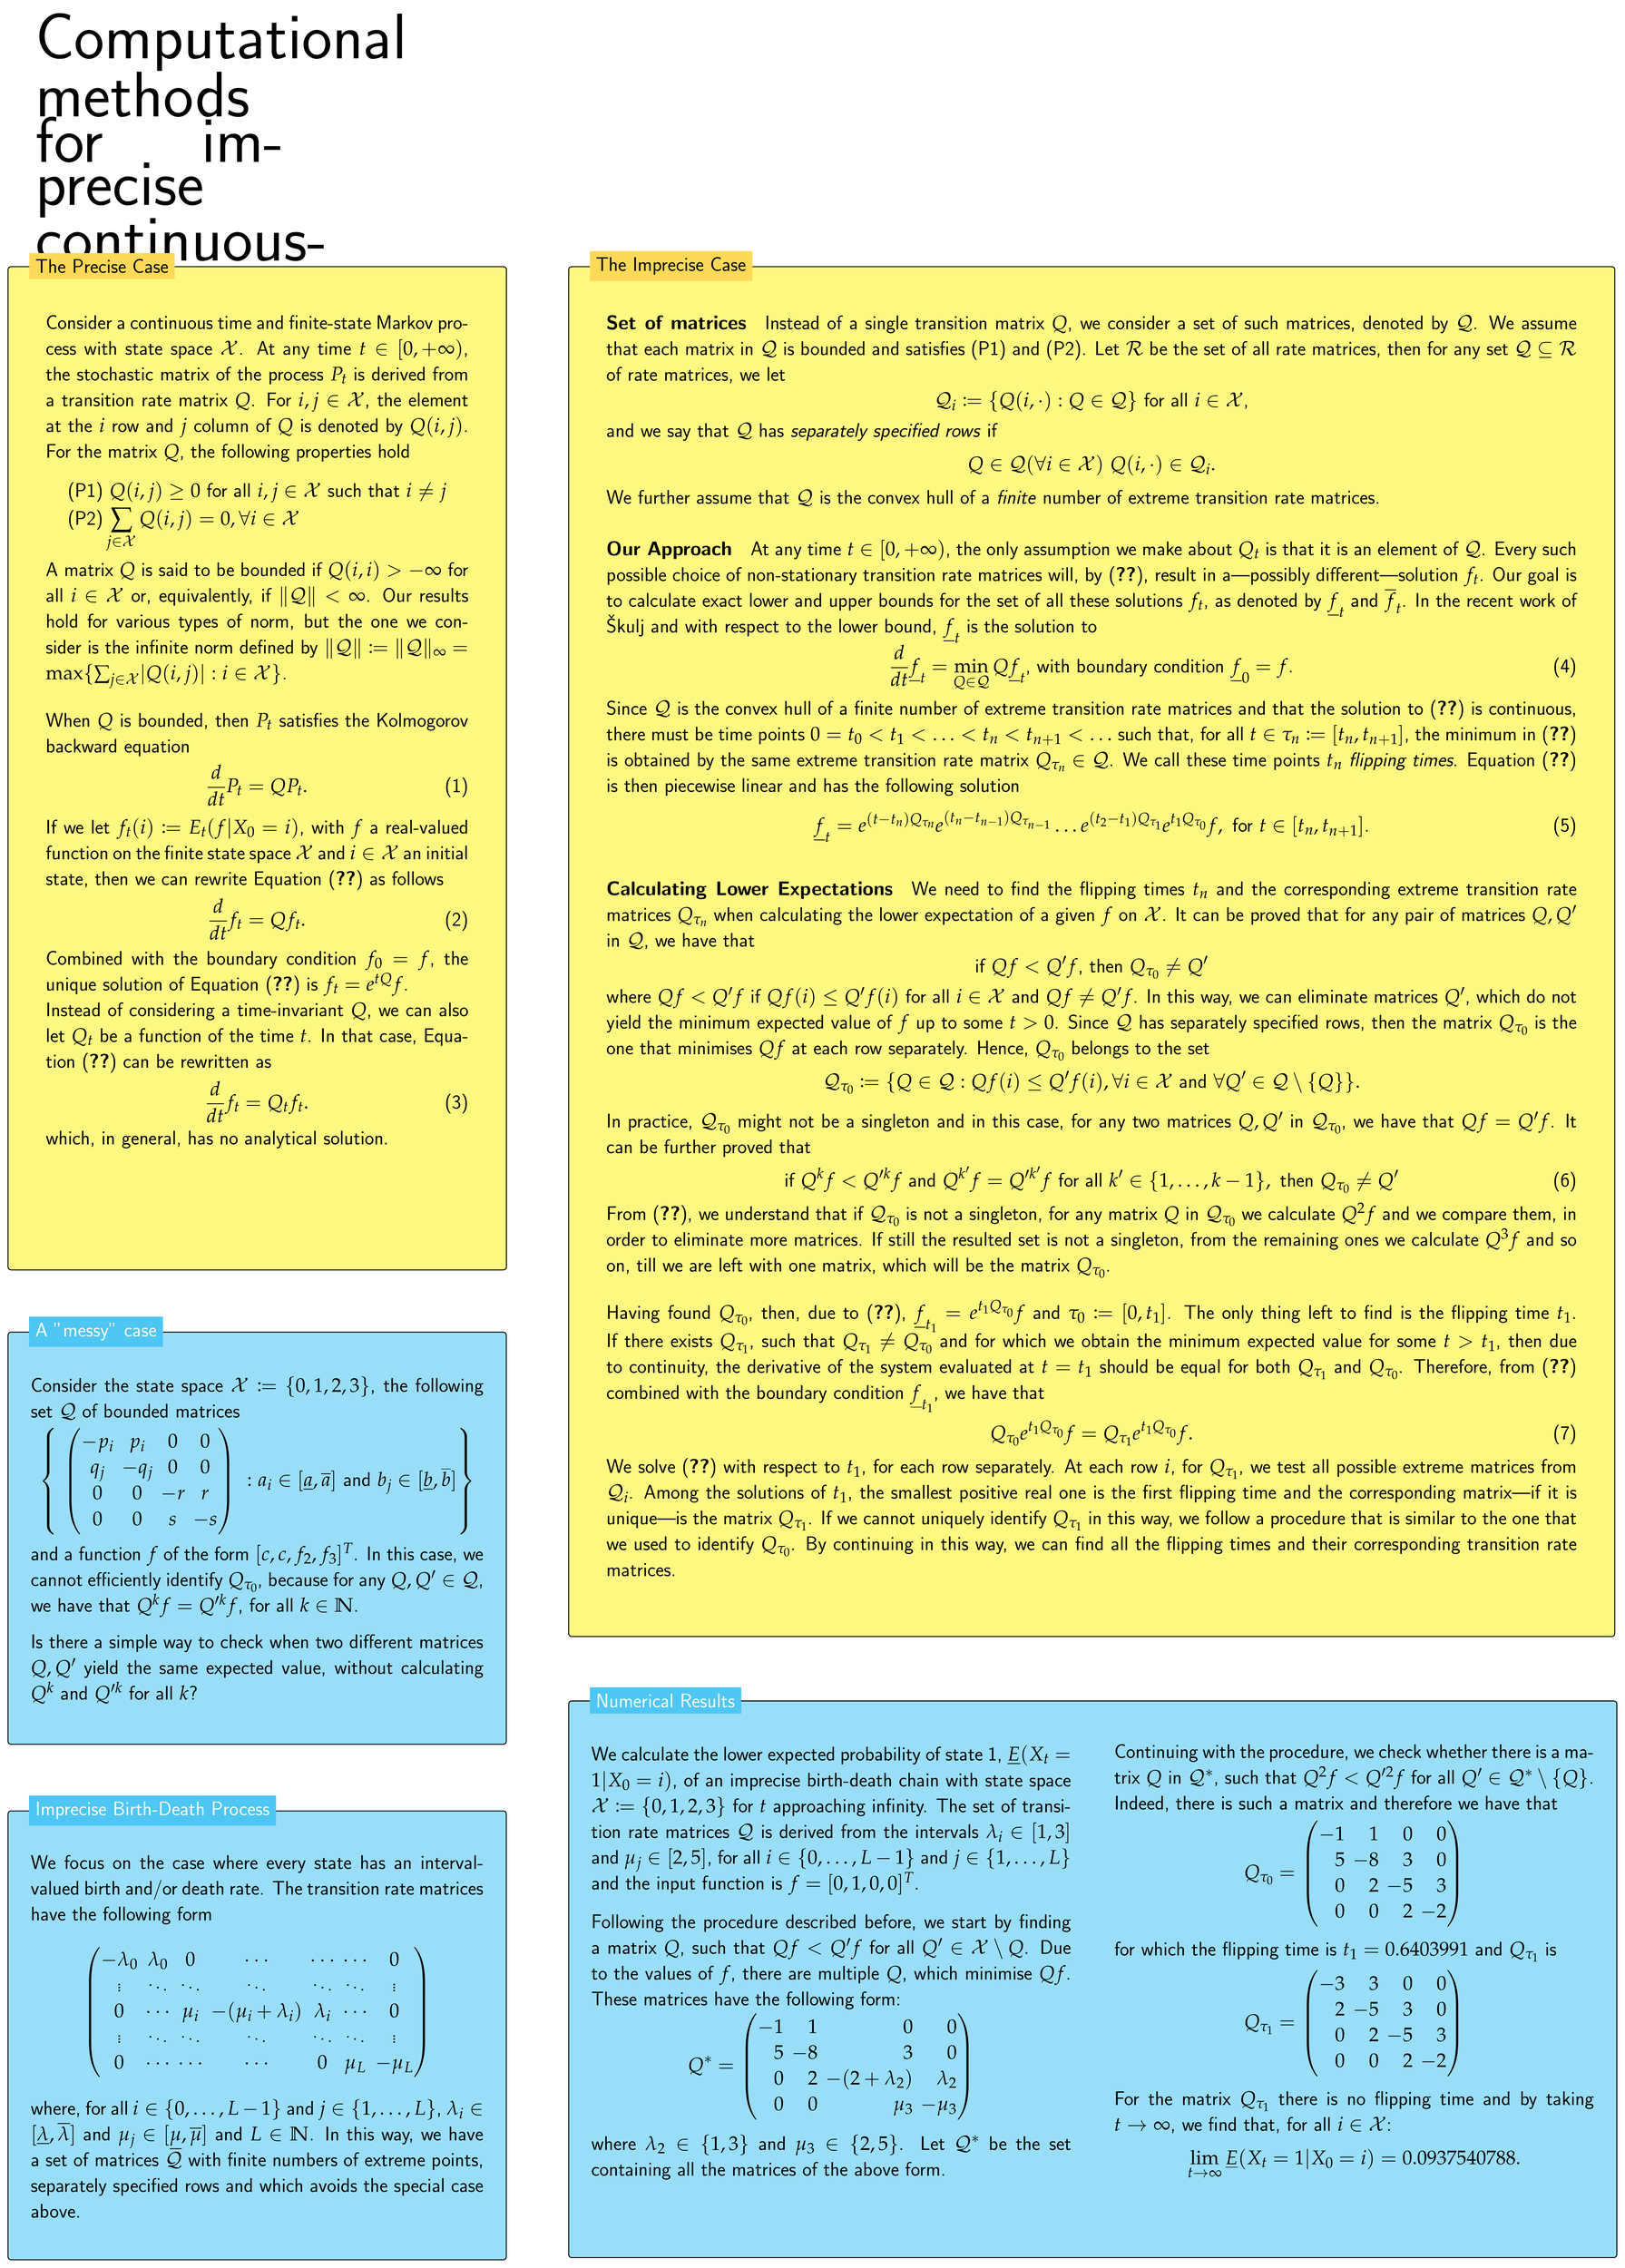
\begin{tikzpicture}
    
    %% teken de achtergrond
    % \begin{pgfonlayer}{background}
    %   \shade[top color=white, bottom color=grey!30!green!10] 
    %        (0cm,113.3cm) rectangle (80cm,0cm); 
    % \end{pgfonlayer}

\tikzstyle{uitleg} = [draw=black, fill=yellow!50, very thick,
    rectangle, rounded corners, inner sep=50pt, inner ysep=50pt]
    \tikzstyle{titel} =[fill=yellow!80!red!65!, text=black]
    \tikzstyle{uitlegmessage} = [draw=black,fill=cyan!40, very thick,
    rectangle, rounded corners, inner sep=30pt, inner ysep=30pt]
    \tikzstyle{titelmessage} = [draw=cyan!70, fill=cyan!70, text=white]
    \tikzstyle{uitlegvb} = [draw=orange!50!yellow, fill=orange!25!white, very thick,
    rectangle, rounded corners, inner sep=50pt, inner ysep=50pt]
    \tikzstyle{titelvb} =[fill=orange!50!yellow, text=white]
    \tikzstyle{uitlegdilation} = [draw=orange!50!yellow, fill=orange!25!white, very thick,
    rectangle, rounded corners, inner sep=50pt, inner ysep=50pt]
    \tikzstyle{titeldilation} =[fill=orange!50!yellow, text=white]

\node[rectangle, anchor=north west] (titel) at (1,111)
     {\begin{minipage}{{.95\textwidth}}
         {\VeryHuge Computational methods for imprecise continuous-time birth-death processes: a preliminary study of flipping times}%\\[.8\baselineskip]
         % \begin{center}
         \hspace{6.8cm}
         {\LARGE\bfseries Stavros Lopatatzidis, Jasper De Bock, Gert de Cooman}
       \end{minipage}
     };


\node[uitleg, anchor=north west] (HMMuitleg) at (0.0,99) {
\begin{minipage}
[t][43cm]
{19.6cm}
\vspace{0.5cm}
Consider a continuous time and finite-state Markov process with state space $\stateset$. 
At any time $t\in[0,+\infty)$, the stochastic matrix of the process $P_{t}$ is derived from a transition rate matrix~$Q$.
%The dimension of both $P_{t}$ and $Q$ is $\abs{\stateset}\times\abs{\stateset}$, where $\abs{\stateset}$ is the cardinality of $\stateset$.
For $i,j\in\stateset$, the element at the $i$ row and $j$ column of $Q$ is denoted by $Q(i,j)$.
For the matrix $Q$, the following properties hold
\vspace{0.4cm}
\begin{equation*}
\begin{split}
&\text{(P1)~}Q(i,j)\geq0\text{ for all } i,j\in\stateset \text{ such that } i\neq j\vspace{5pt}\\
&\text{(P2)}\sum_{j\in\stateset}Q(i,j)=0, \forall i\in\stateset
\end{split}
\end{equation*}
A matrix $Q$ is said to be bounded if $Q(i,i)>-\infty$ for all $i\in\stateset$ or, equivalently, if $\norm{\matrices}<\infty$.
Our results hold for various types of norm, but the one we consider is the infinite norm defined by $\norm{\matrices}\coloneqq\norm{\matrices}_{\infty}=\max\{\sum_{j\in\stateset}\abs{Q(i,j)}: i\in\stateset\}$.
\vspace{1cm}

When $Q$ is bounded, then $P_{t}$ satisfies the Kolmogorov backward equation
\begin{equation} \label{Kol_eq}
\frac{d}{dt}P_{t}=QP_{t}.\vspace{5pt}
\end{equation}
If we let $f_{t}(i)\coloneqq E_{t}(f\vert X_0=i)$, with $f$ a real-valued function on the finite state space~$\mathcal{X}$ and $i\in\mathcal{X}$ an initial state, then 
we can rewrite Equation~\eqref{Kol_eq} as follows
\begin{equation} \label{T_Kol_eq}
\frac{d}{dt}f_{t}=Qf_{t}.
\vspace{3pt}
\end{equation}
Combined with the boundary condition $f_0=f$, the unique solution of Equation~\eqref{T_Kol_eq} is $f_{t}=e^{tQ}f$.

Instead of considering a time-invariant $Q$, we can also let $Q_{t}$ be a function of the time $t$.
 In that case, Equation \eqref{T_Kol_eq} can be rewritten as
 \begin{equation} \label{time_Kol_eq}
\frac{d}{dt}f_{t}=Q_{t}f_{t}. 
\end{equation}
which, in general, has no analytical solution.

\end{minipage}
};
  
\node[titel,right=1cm] at (HMMuitleg.north west) {\titletextsize The Precise Case\vspace{1cm}};

\node[uitleg, anchor=north west] (impreciezeHMMsleren) at (26,99) {
\begin{minipage}
[t][60cm]
{45cm}
\vspace{0.5cm}
\begin{minipage}{45cm}
% Finite-state birth-death chains are special cases of time-homogeneous finite-state Markov chains.
\paragraph{Set of matrices} Instead of a single transition matrix $Q$, we consider a set of such matrices, denoted by  $\matrices$.
We assume that each matrix in $\matrices$ is bounded and satisfies (P1) and (P2).
Let $\mathcal{R}$ be the set of all rate matrices, then for any set $\matrices\subseteq\mathcal{R}$ of rate matrices, we let
\begin{equation*}
\matrices_i\coloneqq\{Q(i,\cdot): Q\in\matrices\}
\text{ for all $i\in\stateset$,}
\end{equation*}
and we say that $\matrices$ has \emph{separately specified rows} if
\begin{equation*}
Q\in\matrices(\forall i\in\stateset)~Q(i,\cdot)\in\matrices_i.
\end{equation*}
We further assume that $\matrices$ is the convex hull of a \emph{finite} number of extreme transition rate matrices.
\vspace{1.2cm}
% For any bounded set $\matrices$ of rate matrices, the corresponding \emph{lower transition rate operator} $\lrate$ is a map from $\gamblesX$ to $\gamblesX$. For all $f\in\gamblesX$, $\lrate f$ is defined by
% \begin{equation}\label{eq:deflowerbound}
% (\lrate f)(x)\coloneqq\inf\{(Qf)(x)\colon Q\in\matrices\}\text{ for all $x\in\stateset$}.
% \end{equation}

%\textbf{row separated, finite number of extreme points}

\paragraph{Our Approach} At any time $t\in[0,+\infty)$, the only assumption we make about $Q_{t}$ is that it is an element of $\mathcal{Q}$. 
Every such possible choice of non-stationary transition rate matrices will, by \eqref{time_Kol_eq}, result in a---possibly different---solution $f_t$. 
Our goal is to calculate exact lower and upper bounds for the set of all these solutions $f_{t}$, as denoted by $\smash{\underline{f}_{t}}$ and $\smash{\overline{f}_{t}}$.
In the recent work of \v{S}kulj and with respect to the lower bound, $\smash{\underline{f}_{t}}$ is the solution to
\begin{equation} \label{ip_Kol_eq}
\frac{d}{dt}\underline{f}_{t}=\min_{Q\in \mathcal{Q}}Q\underline{f}_{t} \text{, with boundary condition $\underline{f}_0=f$.}
\end{equation}
Since $\mathcal{Q}$ is the convex hull of a finite number of extreme transition rate matrices and that the solution to \eqref{ip_Kol_eq} is continuous, there must be time points $0=t_0<t_1<\ldots<t_{n}<t_{n+1}<\ldots$ such that, for all $t\in \tau_{n}\coloneqq[t_n,t_{n+1}]$, the minimum in \eqref{ip_Kol_eq} is obtained by the same extreme transition rate matrix $Q_{\tau_n}\in\mathcal{Q}$. We call these time points $t_n$ \emph{flipping times}. Equation~\eqref{ip_Kol_eq} is then piecewise linear and has the following solution 
\vspace{0.3cm}
\begin{equation} \label{eq:min_lin}
\underline{f}_t=e^{(t-t_n)Q_{\tau_{n}}}e^{(t_n-t_{n-1})Q_{\tau_{n-1}}}\dots e^{(t_2-t_1)Q_{\tau_{1}}}e^{t_1 Q_{\tau_0}}f, \text{ for $t\in[t_n,t_{n+1}]$.}\vspace{0.2cm}
\end{equation}
\vspace{0cm}
\paragraph{Calculating Lower Expectations} We need to find the flipping times $t_n$ and the corresponding extreme transition rate matrices $Q_{\tau_{n}}$ when calculating the lower expectation of a given $f$ on $\stateset$. 
% It is known that
% \begin{equation} \label{eq:der}
% \frac{\partial}{\partial t}\bigl[e^{tQ}f\bigr]\Big\vert_{t=0}=Qf \Rightarrow (\forall\ve>0)(\exists \de>0)(\forall t \in(0,\de))\norm{e^{tQ}f-f-tQf}_{\infty}<t\ve
% \end{equation}
It can be proved that for any pair of matrices $Q, Q'$ in $\matrices$, we have that
\begin{equation*}
\text{if $Qf < Q'f$, then }Q_{\tau_{0}}\neq Q'
\end{equation*}
where $Qf<Q'f\text{ if } Qf(i)\leq Q'f(i) \text{ for all $i\in\stateset$ and } Qf\neq Q'f$.
%In order to find $Q_{\tau_{0}}$ in \eqref{eq:min_lin}, we need to find a $Q$ such that $Qf<Q'f$, for all $Q'\in\matrices\setminus\{Q\}$.
In this way, we can eliminate matrices $Q'$, which do not yield the minimum expected value of $f$ up to some $t>0$.  
Since $\matrices$ has separately specified rows, then the matrix $Q_{\tau_{0}}$ is the one that minimises $Qf$ at each row separately.
Hence, $Q_{\tau_{0}}$ belongs to the set 
\begin{equation*}
\matrices_{\tau_{0}}\coloneqq\{Q\in\matrices : Qf(i)\leq Q'f(i), \forall i\in\stateset \text{ and } \forall Q'\in\matrices\setminus\{Q\}\}.
\vspace{0.3cm}
\end{equation*}
% Hence, there is $t$, small enough, such that 
% First of all, the value of $e$blabla can be identified by its $k-$derivative at time 0.
In practice, $\matrices_{\tau_{0}}$ might not be a singleton and in this case, for any two matrices $Q,Q'$ in $\matrices_{\tau_{0}}$, we have that $Qf=Q'f$.
It can be further proved that 
\begin{equation} \label{eq:derk}
\text{if } Q^{k}f<Q'^{k}f \text{ and } Q^{k'}f=Q'^{k'}f \text{ for all } k'\in\{1,\ldots,k-1\},\text{ then }Q_{\tau_{0}}\neq Q'
\end{equation}
From \eqref{eq:derk}, we understand that if $\matrices_{\tau_{0}}$ is not a singleton, for any matrix $Q$ in $\matrices_{\tau_{0}}$ we calculate $Q^{2}f$ and we compare them, in order to eliminate more matrices.
If still the resulted set is not a singleton, from the remaining ones we calculate $Q^{3}f$ and so on, till we are left with one matrix, which will be the matrix $Q_{\tau_{0}}$.
%Therefore, if $\matrices_{\tau_{0}}$ is not a singleton, then $Q_{\tau_{0}}$ is a single matrix $Q$ of $\matrices_{\tau_{0}}$, for which \eqref{eq:derk} holds.
\vspace{1cm}

Having found $Q_{\tau_{0}}$, then, due to \eqref{eq:min_lin}, $\underline{f}_{t_1}=e^{t_{1}Q_{\tau_{0}}}f$ and $\tau_{0}\coloneqq[0,t_1]$.
The only thing left to find is the flipping time $t_1$.
If there exists $Q_{\tau_{1}}$, such that $Q_{\tau_{1}}\neq Q_{\tau_{0}}$ and for which we obtain the minimum expected value for some $t>t_1$, then due to continuity, the derivative of the system evaluated at $t=t_1$ should be equal for both $Q_{\tau_{1}}$ and $Q_{\tau_{0}}$.
Therefore, from \eqref{time_Kol_eq} combined with the boundary condition $\underline{f}_{t_1}$, we have that
% \begin{equation*} %\label{eq:der_t1}
% \frac{\partial}{\partial t}\bigl[e^{tQ}\underline{f}_{t_1}\bigr]\Big\vert_{t=0}=Q\underline{f}_{t_1} = Qe^{t_{1}Q_{\tau_{0}}}f
% \end{equation*}
% and due to continuity, 
\begin{equation} \label{eq:flip1}
Q_{\tau_{0}}e^{t_{1}Q_{\tau_{0}}}f = Q_{\tau_{1}}e^{t_{1}Q_{\tau_{0}}}f.
\end{equation}
We solve \eqref{eq:flip1} with respect to $t_1$, for each row separately.
At each row $i$, for $Q_{\tau_{1}}$, we test all possible extreme matrices from $\matrices_i$. 
Among the solutions of $t_1$, the smallest positive real one is the first flipping time and the corresponding matrix---if it is unique---is the matrix $Q_{\tau_{1}}$.
If we cannot uniquely identify $Q_{\tau_{1}}$ in this way, we follow a procedure that is similar to the one that we used to identify $Q_{\tau_{0}}$. By continuing in this way, we can find all the flipping times and their corresponding transition rate matrices.
\end{minipage}

%Similarly, we use $\state{1:\infty}$ as a shorthand notation for the infinite sequence $\state{1},\ldots,\state{n},\ldots$ Also, for every $k\in\nats$ such that $k\leq n$, we let $\state{k:n}$ and $\state{k:\infty}$ be the sequences of states from time point $k$ to $n$ or infinity, respectively.
% \end{minipage}

% \begin{minipage}{49cm}
% \vspace{0.5cm}
% \begin{multicols}{2}
% \paragraph{Different Types of Independence} 
% Hence, the remaining waiting time of the last item in the queue would have the same bounds by using either epistemic independence or strong independence.\\

% \paragraph{Experimental Work} We also provide some experimental results regarding the lower and upper prevision of the number of items in the queue ($\overline{\underline{P}}(X_{t})$), the number of items in the queue conditional on an entrance ($\overline{\underline{P}}(X_{t}|entr)$) and the remaining waiting time of the last item conditional on an entrance ($\overline{\underline{P}}(W_{t}|entr)$), as $t \to \infty$. \\
% \end{multicols}
% \end{minipage}

\end{minipage}
};


\node[titel,right=1cm] at (impreciezeHMMsleren.north west) {\titletextsize The Imprecise Case};


\node[uitlegmessage, anchor=north west] (propertiesTransMod) at (0.0,49.6){
\begin{minipage}[t][17cm]{21cm}
\vspace{1cm}

Consider the state space $\stateset\coloneqq\{0,1,2,3\}$, the following set $\matrices$ of bounded matrices 
\begin{equation*}
\left\{\text{
$
 \begin{pmatrix*}
  -p_i & p_i & 0 & 0 \\
  q_j & -q_j & 0 & 0\\
  0 & 0 & -r & r \\
  0 & 0 & s & -s 
  \end{pmatrix*}$
  }:
  a_i\in[\underline{a},\overline{a}]\text{ and }b_j\in[\underline{b},\overline{b}]\right\}
\end{equation*}
and a function $f$ of the form $[c,c,f_{2},f_{3}]^T$.
In this case, we cannot efficiently identify $Q_{\tau_{0}}$, because for any $Q,Q'\in\matrices$, we have that $Q^{k}f=Q'^{k}f$, for all $k\in\nats$.
\vspace{0.5cm}

Is there a simple way to check when two different matrices $Q,Q'$ yield the same expected value, without calculating $Q^k$ and $Q'^k$ for all $k$?
\end{minipage}
};

\node[titelmessage,right=1cm] at (propertiesTransMod.north west) {\titletextsize A "messy" case};


\node[uitlegmessage, anchor=north west] (propertiesTransMod) at (0.0,27.4){
\begin{minipage}[t][18.7cm]{21cm}
\vspace{1cm}
We focus on the case where every state  
has an interval-valued birth and/or death rate. The transition rate matrices have the following form

\begin{equation*}
 \begin{pmatrix}
  -\lambda_{0} & \lambda_{0} & 0 & \cdots & \cdots & \cdots & 0 \\
  \vdots & \ddots & \ddots & \ddots & \ddots & \ddots & \vdots  \\
  0 & \cdots & \mu_{i} & -(\mu_{i}+\lambda_{i}) & \lambda_{i} & \cdots & 0 \\
  \vdots & \ddots & \ddots & \ddots & \ddots & \ddots & \vdots  \\
  0 & \cdots & \cdots &\cdots & 0 & \mu_{L} & -\mu_{L}
 \end{pmatrix}
\end{equation*}
\vspace{0.3cm}

where, for all $i\in\{0,\dots,L-1\}$ and $j\in\{1,\dots,L\}$, $\lambda_{i} \in [\underline{\lambda},\overline{\lambda}]$ and $\mu_{j} \in [\underline{\mu},\overline{\mu}]$ and $L \in\nats$.
In this way, we have a set of matrices $\matrices$ with finite numbers of extreme points, separately specified rows and which avoids the special case above. 

\end{minipage}
};

\node[titelmessage,right=1cm] at (propertiesTransMod.north west) {\titletextsize Imprecise Birth-Death Process};


\node[uitlegmessage,anchor=north west] (dilation) at (26,32.5){
\begin{minipage}[t][23.7cm]{46.5cm}
\begin{multicols}{2}
\vspace*{1cm}
We calculate the lower expected probability of state 1, $\underline{E}(X_{t}=1\vert X_0=i)$, of an imprecise birth-death chain with state space $\stateset\coloneqq\{0,1,2,3\}$ for $t$ approaching infinity.  
The set of transition rate matrices $\mathcal{Q}$ is derived from the intervals $\lambda_i \in[1,3]$ and $\mu_j \in [2,5]$, for all $i\in\{0,\dots,L-1\}$ and $j\in\{1,\dots,L\}$ and the input function is $f=[0,1,0,0]^T$.\\[-6mm]

Following the procedure described before, we start by finding a matrix $Q$, such that $Qf<Q'f$ for all $Q'\in\stateset\setminus Q$.
Due to the values of $f$, there are multiple $Q$, which minimise $Qf$. 
These matrices have the following form: 
\vspace{-0.2cm}
  \[
  Q^{*}= 
 \begin{pmatrix*}[r]
  -1 & 1 & 0 & 0 \\
  5 & -8 & 3 & 0 \\
  0 & 2 & -(2+\lambda_{2}) & \lambda_{2} \\
  0 & 0 & \mu_{3} & -\mu_{3} 
 \end{pmatrix*}
 \vspace{0.3cm}
 \]
 % \[
 %    \begin{pmatrix*}[r]
 %        -1 & 1 & -2\\
 %        0 & -1 & 4\\
 %        0 & 0 & 1
 %    \end{pmatrix*}
 % \]
 where $\lambda_{2}\in\{1,3\}$ and $\mu_{3}\in\{2,5\}$. Let $\matrices^*$ be the set containing all the matrices of the above form.
 %, as we can consider only the extreme points of the respective rate intervals. 
 \columnbreak

~
\vspace{4mm}
~\\
 Continuing with the procedure, we check whether there is a matrix $Q$ in $\matrices^*$, such that $Q^{2}f<Q'^{2}f$ for all $Q'\in\matrices^{*}\setminus\{Q\}$. 
 Indeed, there is such a matrix and therefore we have that
\[ 
 Q_{\tau_{0}} =
 \begin{pmatrix*}[r]
  -1 & 1 & 0 & 0 \\
  5 & -8 & 3 & 0 \\
  0 & 2 & -5 & 3 \\
  0 & 0 & 2 & -2 
 \end{pmatrix*}
 \vspace{0.3cm}
\]
 for which the flipping time is $t_{1}=0.6403991$ and $Q_{\tau_{1}}$ is
 \[
 Q_{\tau_{1}}= 
 \begin{pmatrix*}[r]
  -3 & 3 & 0 & 0 \\
  2 & -5 & 3 & 0 \\
  0 & 2 & -5 & 3 \\
  0 & 0 & 2 & -2 
 \end{pmatrix*}
  \vspace{0.3cm}
\]
% (from Q0b) Q1 := Matrix([[-3,3,0,0],[2,-5,3,0],[0,2,-5,3],[0,0,2,-2]])
% Matrix(4, 1, {(1, 1) = 0.9375407882e-1+0.25274635e-3*exp(-8.464101615*t)-0.929433068e-2*exp(-5.*t)+0.2886413789e-1*exp(-1.535898385*t), (2, 1) = -0.46034388e-3*exp(-8.464101615*t)+0.9375407874e-1+0.619622048e-2*exp(-5.*t)+0.1408667698e-1*exp(-1.535898385*t), (3, 1) = 0.619622043e-2*exp(-5.*t)+0.36306168e-3*exp(-8.464101615*t)+0.9375407880e-1-0.2976865208e-2*exp(-1.535898385*t), (4, 1) = -0.1282850569e-1*exp(-1.535898385*t)-0.413081362e-2*exp(-5.*t)-0.11233166e-3*exp(-8.464101615*t)+0.9375407877e-1})
% no flipping time t2
%lower prob = 0.0937540788
For the matrix $Q_{\tau_{1}}$ there is no flipping time and by taking $t\to\infty$, we find that, for all $i\in\mathcal{X}$:
\begin{equation*}
\lim_{t\to\infty}\underline{E}(X_t=1\vert X_0=i) = 0.0937540788.
\end{equation*}
\end{multicols}
\end{minipage}
};
\node[titelmessage,right=1cm] at (dilation.north west) {\titletextsize Numerical Results};





\end{tikzpicture}
\end{center}

\end{document}